\section{Supplemental Figures}
\newpage

\begin{figure}[H]
  \centering
  \caption{Ordination of Bray-Curtis sample pairwise distances for each incubation time. Point area is proportional to the density of the CsCl gradient fraction for each sequence library, and color/shape reflects control (red triangles) or labeled (blue circles) treatment. Inset shows Bray-Curtis distances for paired control versus labeled CsCl gradient fractions (i.e. fractions from the same incubation day and same density) against the density of the pair (p-value: 4.526e$^{-5}$, r$^{2}$: 0.434).}
  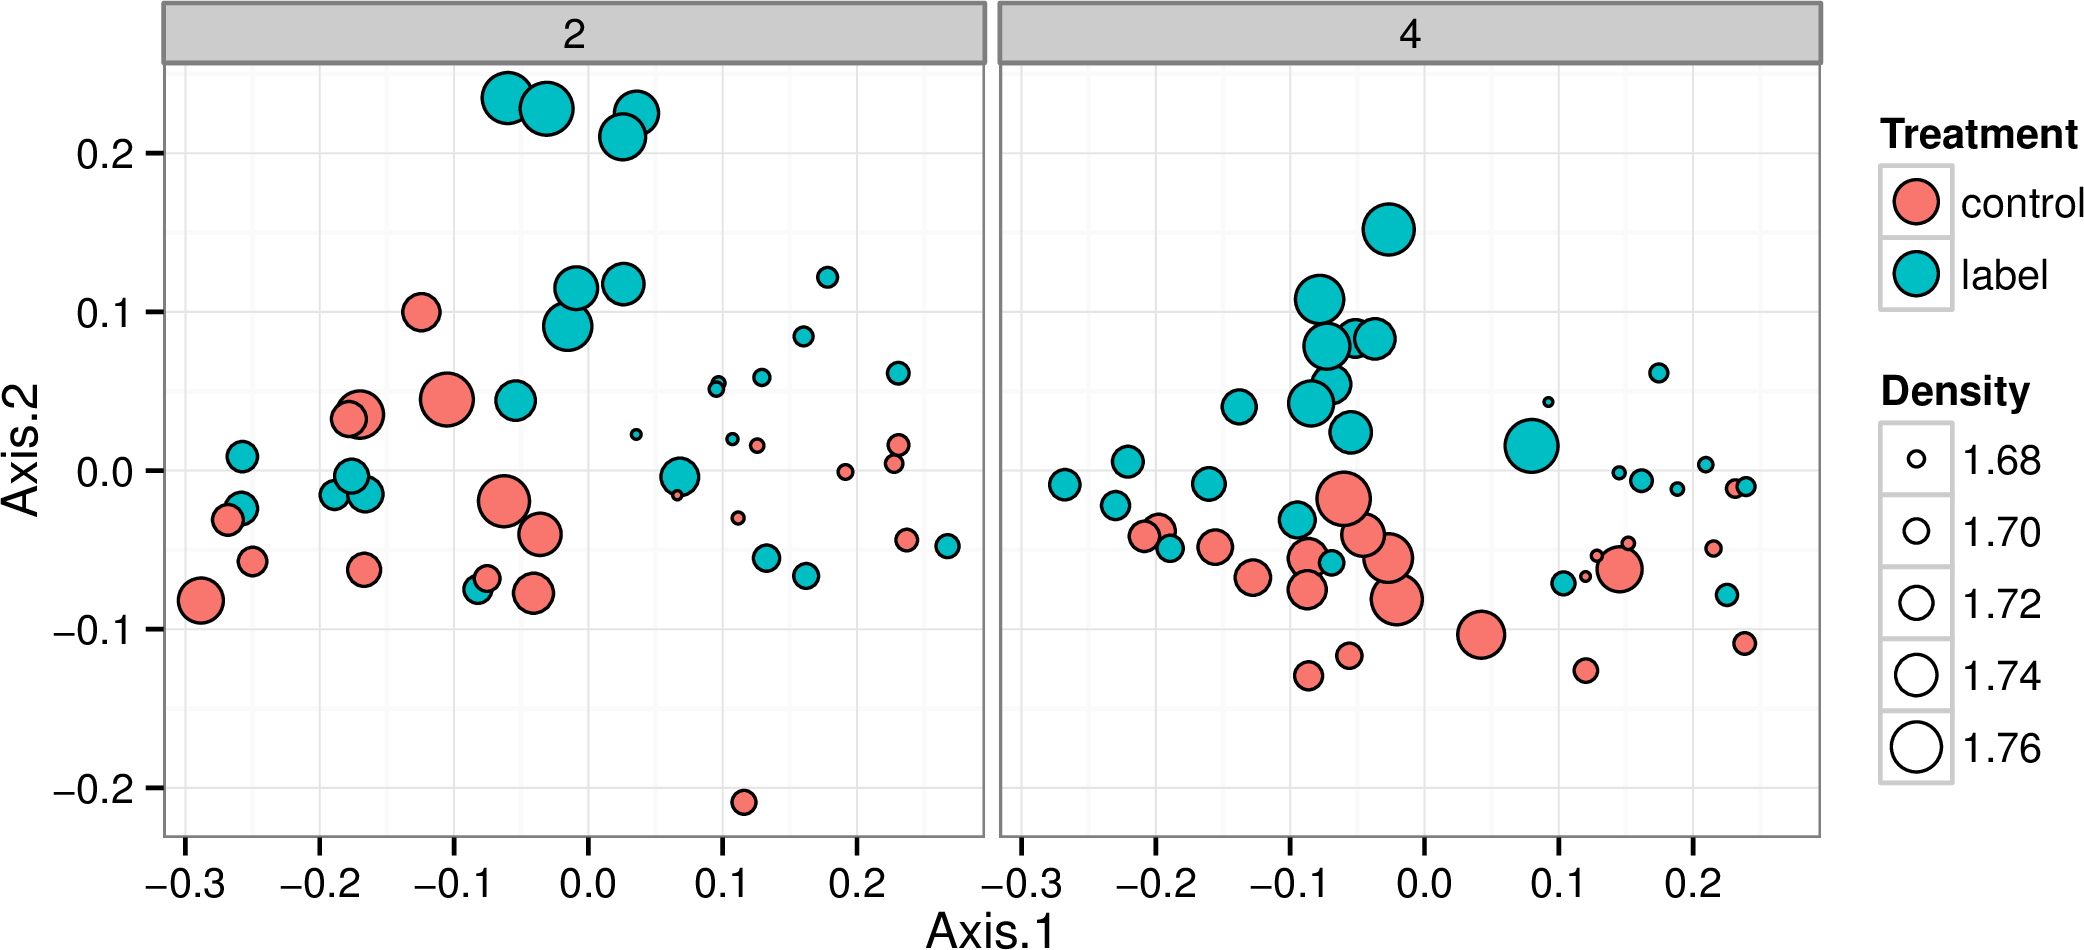
\includegraphics[width=1.0\textwidth]{figures/ordination_all_day_facet/ordination_all_day_facet.png}
  \label{fig:ordination}
\end{figure}

\begin{figure}[h!]
  \centering
  \caption{Distribution of sequences into top 9 phyla (phyla ranked by sum of all sequence annotations).}
    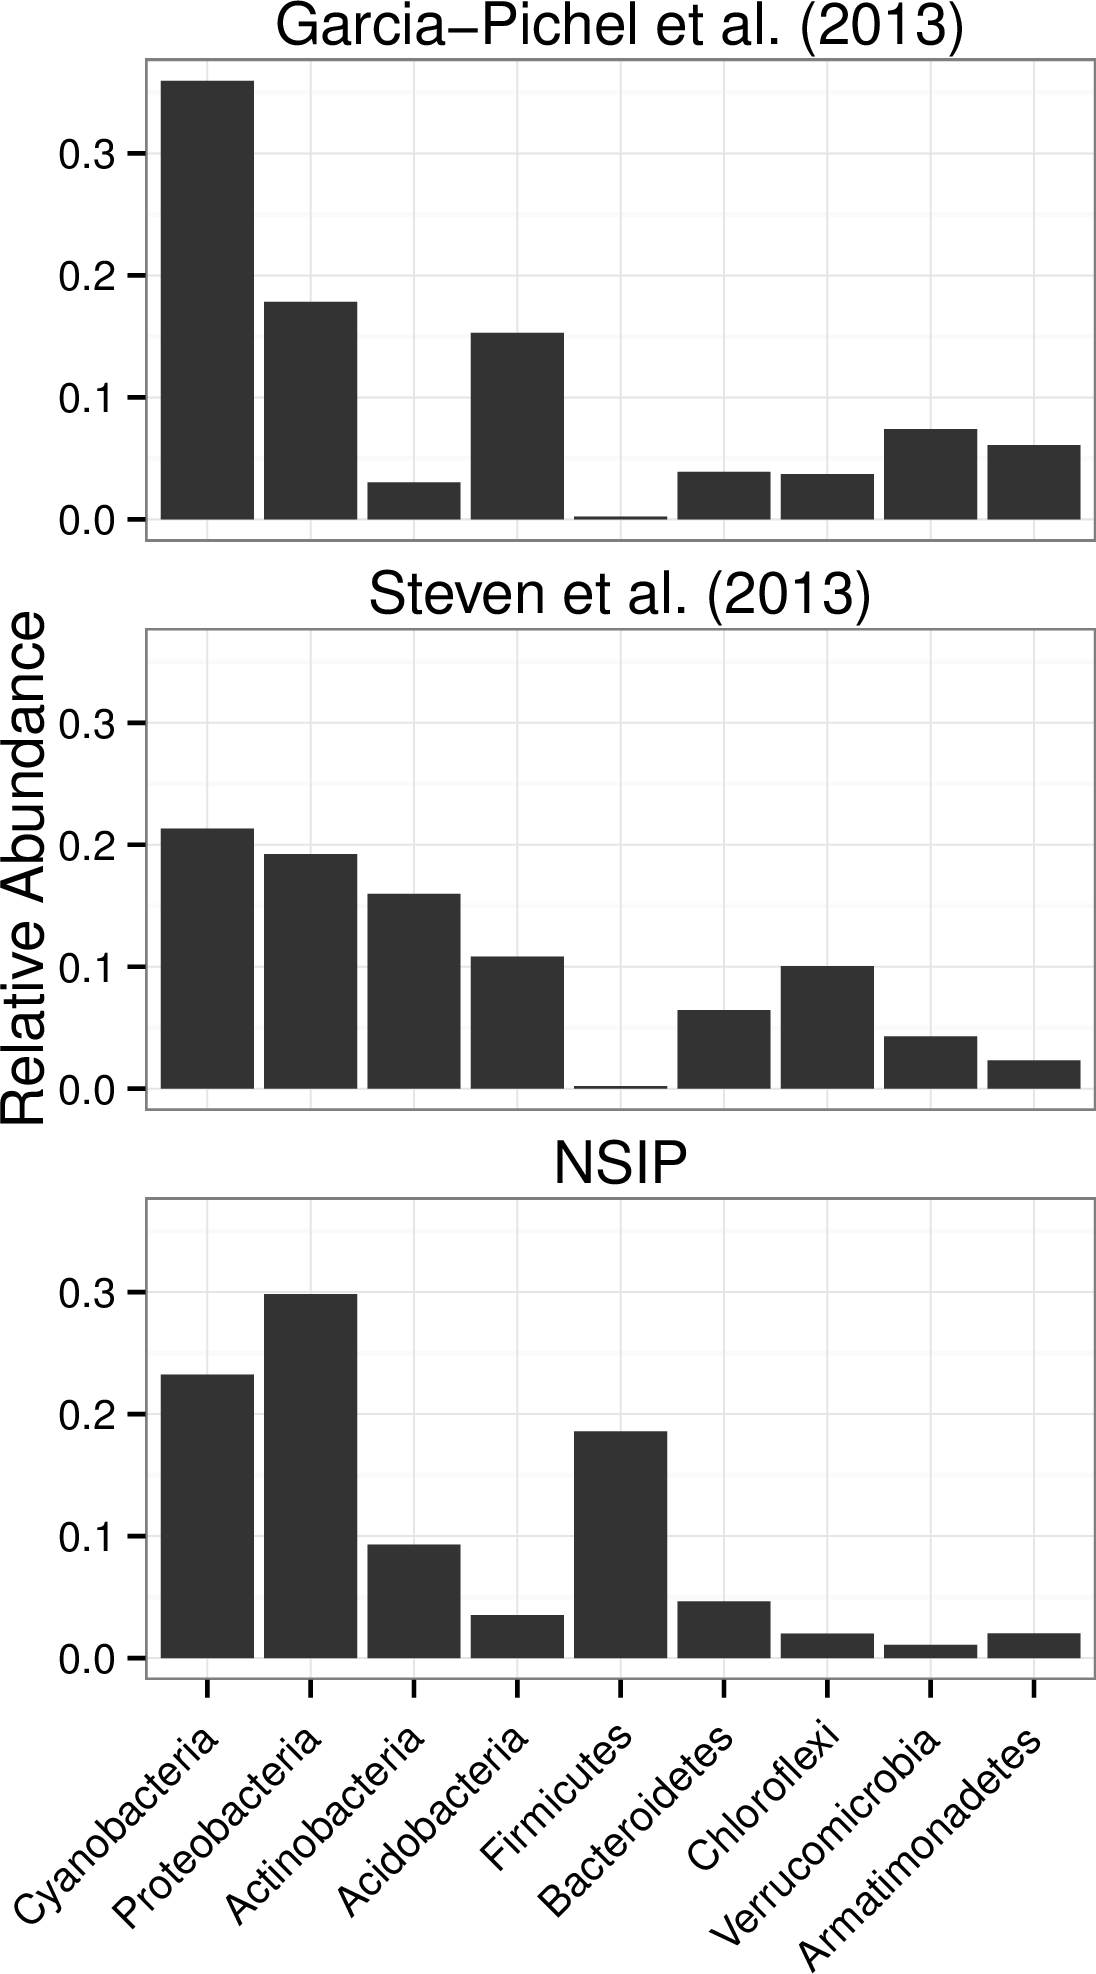
\includegraphics[width=0.5\textwidth]{figures/study_phylum_dist/study_phylum_dist.png}
  \label{fig:study_phy_dist}
\end{figure}

\begin{figure}[H]
  \centering
  \caption{Relative abundance of selected heterocystous cyanobacterial OTUs with centroids from sequences described in \citet{Yeager} (see methods for selection criteria) in \citet{Steven_2013} data set.}
    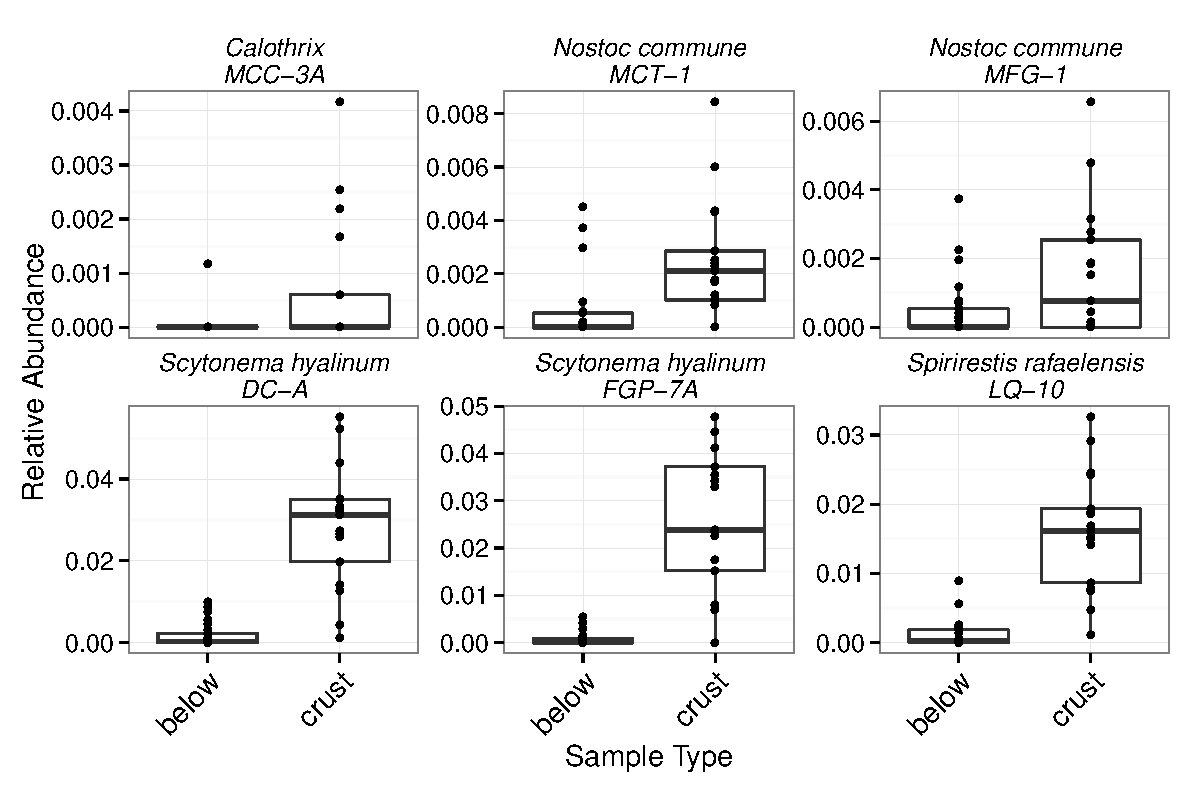
\includegraphics[width=1.0\textwidth]{figures/het_cyano_steven2013/het_cyano_steven2013.pdf}
  \label{fig:het_steven}
\end{figure}

\begin{figure}[H]
  \centering
  \caption{Rarefaction curves for all samples presented by \citet{Garcia_Pichel_2013} and \citet{Steven_2013}. Inset is boxplot of estimated sampling effort for all samples in \citet{Garcia_Pichel_2013} and \citet{Steven_2013} (number of observed OTUs divided by number of CatchAll \cite{BUNGE_2010} estimated total OTUs)}
    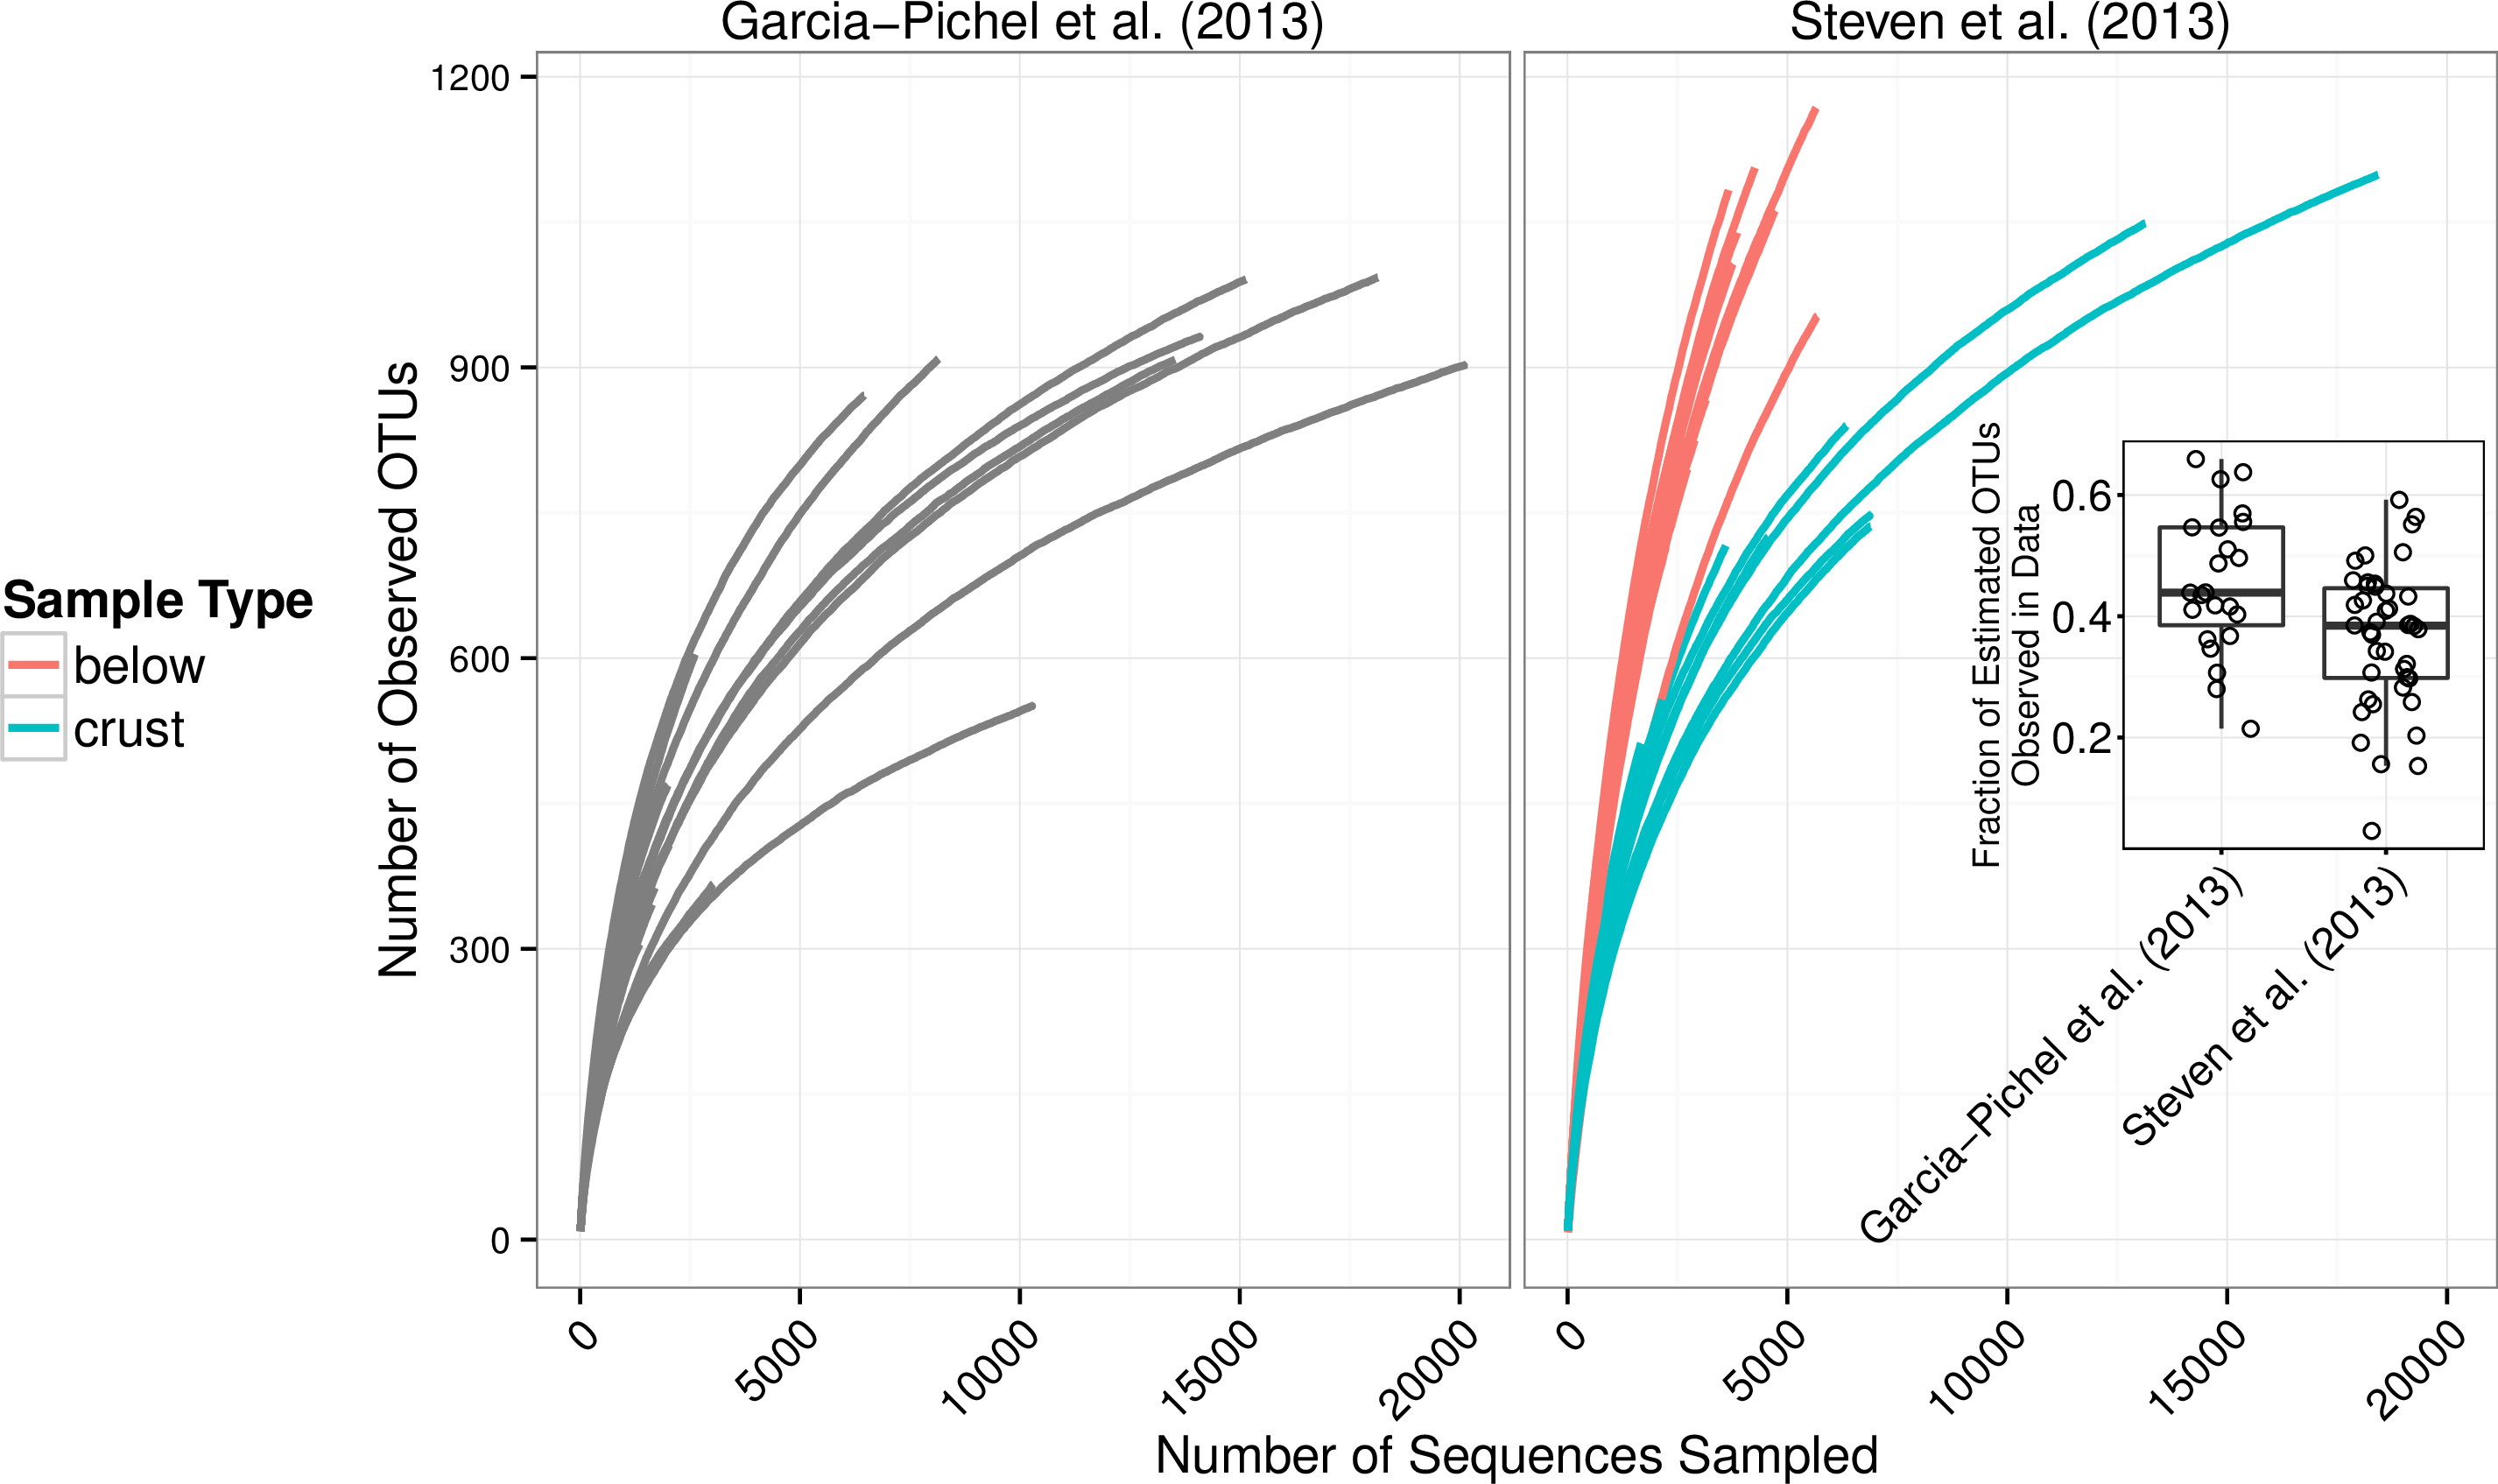
\includegraphics[width=1.0\textwidth]{figures/rarefacation_curves1/raref_and_boxplot.png}
  \label{fig:rarefaction}
\end{figure}

\begin{figure}[H]
  \centering
  \caption{Counts of "responder" OTU occurrences in samples from \citet{Steven_2013} and \citet{Garcia_Pichel_2013}. \citet{Steven_2013} collected BSC samples (25 samples total) and samples from soil beneath BSC (17 samples total, "below" column in figure). \citet{Garcia_Pichel_2013} collected samples from "dark" (9 samples total) and "light" (12 samples total) crusts in addition to "lichen" (2 samples total) dominated crusts.}
    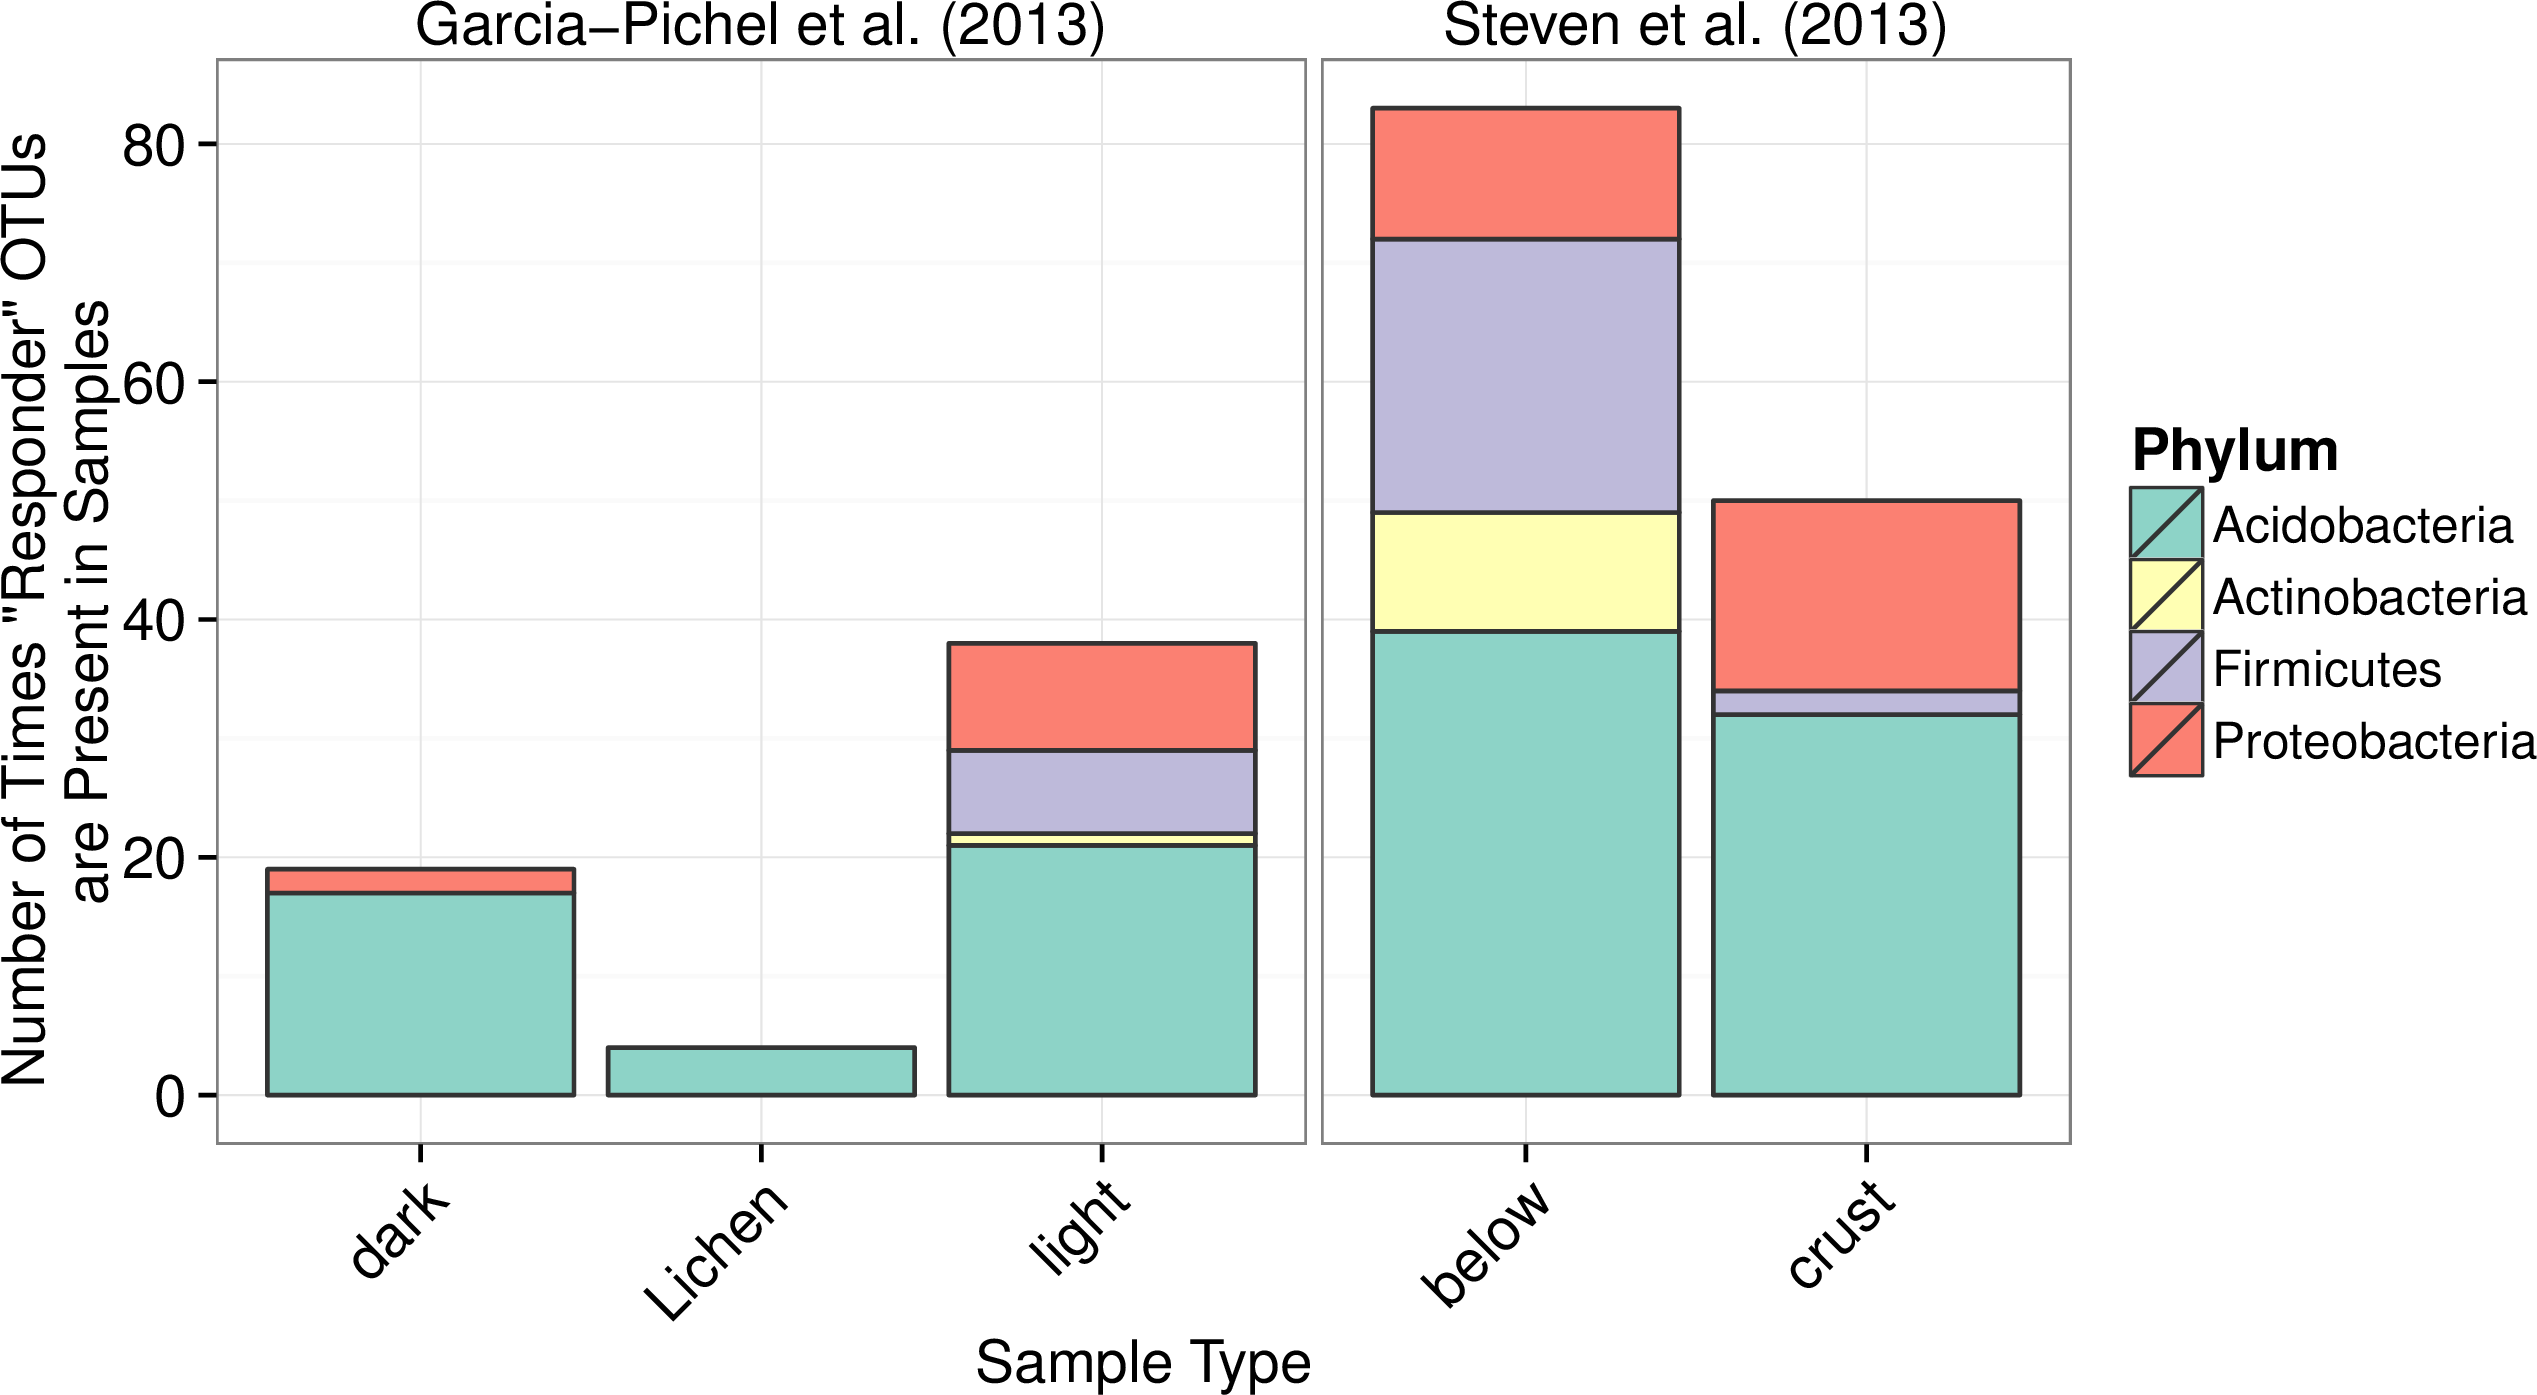
\includegraphics[width=0.8\textwidth]{figures/rspndr_dist/rspndr_dist.png}
  \label{fig:rspndr_dist}
\end{figure}
